\chapter{Studying intercalation}

The project discussed in this section deals with the characterization of the processes at a single electrode. The most efficient method for storing energy is through ion intercalation between atomic layers of an inorganic material. Here we used Lithium titanium phosphate as active material as negative electrode for aqueous sodium-ion batteries.  As for the previous project, the material was produced by Dr. Nicolò Pianta in the research framework of next generation sodium-ion batteries in the group of Profesor Riccardo Ruffo in the University of Milano Bicocca. The non-stationary impedance of the electrode was estimated during constant current and voltage-sweep drifts. The difference between the two is analyzed as well as a physical interpretation. The results of this project led to the publication to a peer-reviewed article [???].

\subsection{Materials and cell assembly}
The project discussed in this section deals with the characterization of the processes at a single electrode. The most efficient method for storing energy is through ion intercalation between atomic layers of an inorganic material. Here we used Lithium titanium phosphate as active material as negative electrode for aqueous sodium-ion batteries.  As for the previous project, the material was produced by Dr. Nicolò Pianta in the research framework of next generation sodium-ion batteries in the group of Profesor Riccardo Ruffo in the University of Milano Bicocca. The non-stationary impedance of the electrode was estimated during constant current and voltage-sweep drifts. The difference between the two is analyzed as well as a physical interpretation. The results of this project led to the publication to a peer-reviewed article [???].
\marginpar{
    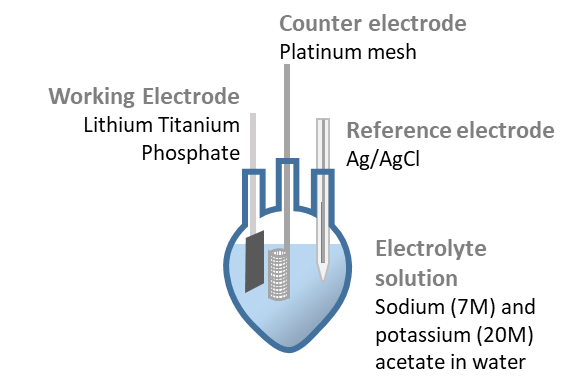
\includegraphics[width=\marginparwidth]{figures/application2/image1.png}
}

\subsection{Measurement set-up}
For this project we used the set-up Version 1 (see page ???) connecting the cell with the potentiostat as a three electrode measurement. In fact, in this case we where only interested in the impedance of one electrode. The connections of cells and devices are reported in figure???.
\marginpar{
    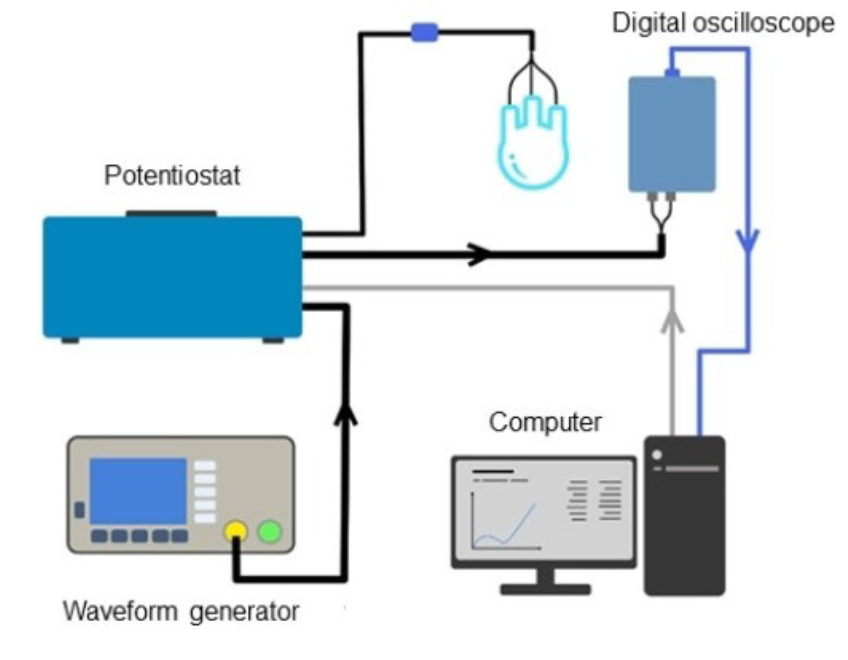
\includegraphics[width=\marginparwidth]{figures/application2/image2.png}
}
We used the same multi-sine of the previous project (see page ???) with a frequency band between 100mHz and 10kHz, sine components amplitude extracted from an EIS experiment and phases selected randomly to minimize the crest factor (the design of multi-sine perturbation is described in ???). The difference here, is the choice of the drift. We superimposed the multi-sine to a cyclic-voltammetry experiment and a galvanostatic experiment. For the former technique we used a scan rate of 0.8 mV/s that correspond of a period of about two hours for a direct comparison of the latter technique in which we used a current of 138mA/g equivalent to a 1C current rate. The multi-frequency current and voltage signals were sampled at a frequency of 50kHz and store in the storage of the computer. The total amount of points was ??? which contains an integer number of multisine periods.

\subsection{Physical model for intercalation}
The electrode under study in this project is mode of an active material for ion intercalation and presents a macroscopic porosity. To model it impedance we selected an intercalation model and applied to the Levi’s theory of porous electrodes. The intercalation

\subsection{Results and discussions}
We estimated the impedance from the multi-frequency voltage and current signals through a Dynamic Multi-Frequency Analysis. We set a bandwidth of 0.1 Hz of the symmetric Fermi-Dirac filter with an n value of 8. A first qualitative analysis of the result of the experiment gives already quite a hint on the previous of intercalation systems. The time-varying impedance during galvanostatic and voltammetry experiments is reported in figure???.
\begin{fullwidth}
    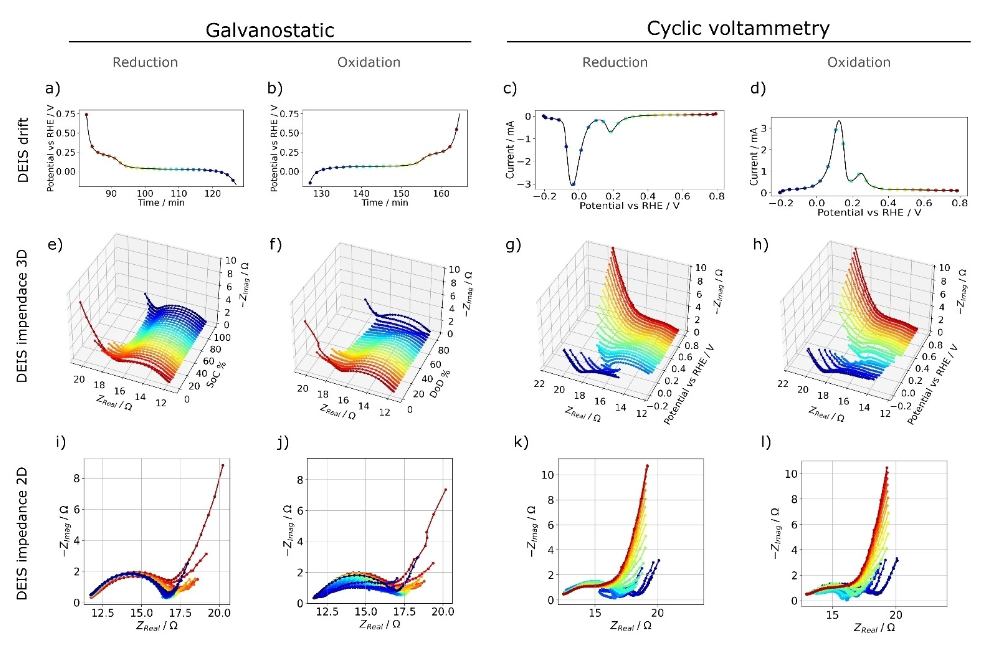
\includegraphics[width=\linewidth]{figures/application2/image3.png}
\end{fullwidth}
It is firstly interesting to se how different they look. The impedance remains of a similar shape

The second curious observation is the asymmetry when inverting the current sign. This characteristics was not observed in the previous project where the double-layer capacitor was tested. It suggests an asymmetry in intercalating and deintercalating ions and the energy necessary to adsorb or desorb them. Continue with the argumentation

\newpage
\section{Comment}
The previous two sections describe two measurement on distinct energy storage devices with the scope of demonstrating the utility of non-stationary impedance for the study of such category of devices and justify the further development. In fact, the technical aspect for the estimation of the impedance are non-trivial. Multi-sine design, signal generation, signal sampling, cell geometry and reference electrode chemistry and placement are too be all carefully considered at the same time. There is a need to understand the physics of the system to deduct the parameter for the measurement. Knowledge of the electronics of potentiostat is fundamental as well as numerical computation and automation via software (i.e. coding). The observation from the results of this two projects were very promising. The following development is the measurement of non-stationary impedance of batteries and its use for the identification of aging. This is the reason why no in-depth study of the electrochemsitry of porous activate carbon and carbon-coated lithim titanium phosphate was continued.  Nevertheless I hope that this preliminary work might inspire scientist interested in mechanistic understanding of such system of replicate our methodology.